% Results

\subsection{Qualitative assessment of vessel underestimation}
\label{subsec:qualitative}

% \begin{figure}[htbp] 
% [htbp] = placement suggestion “try Here, otherwise Top, Bottom, or a dedicated Page" in that order
% \begin{figure}[H] 
% H = “Here definitely”, requires \usepackage{float}
% \centering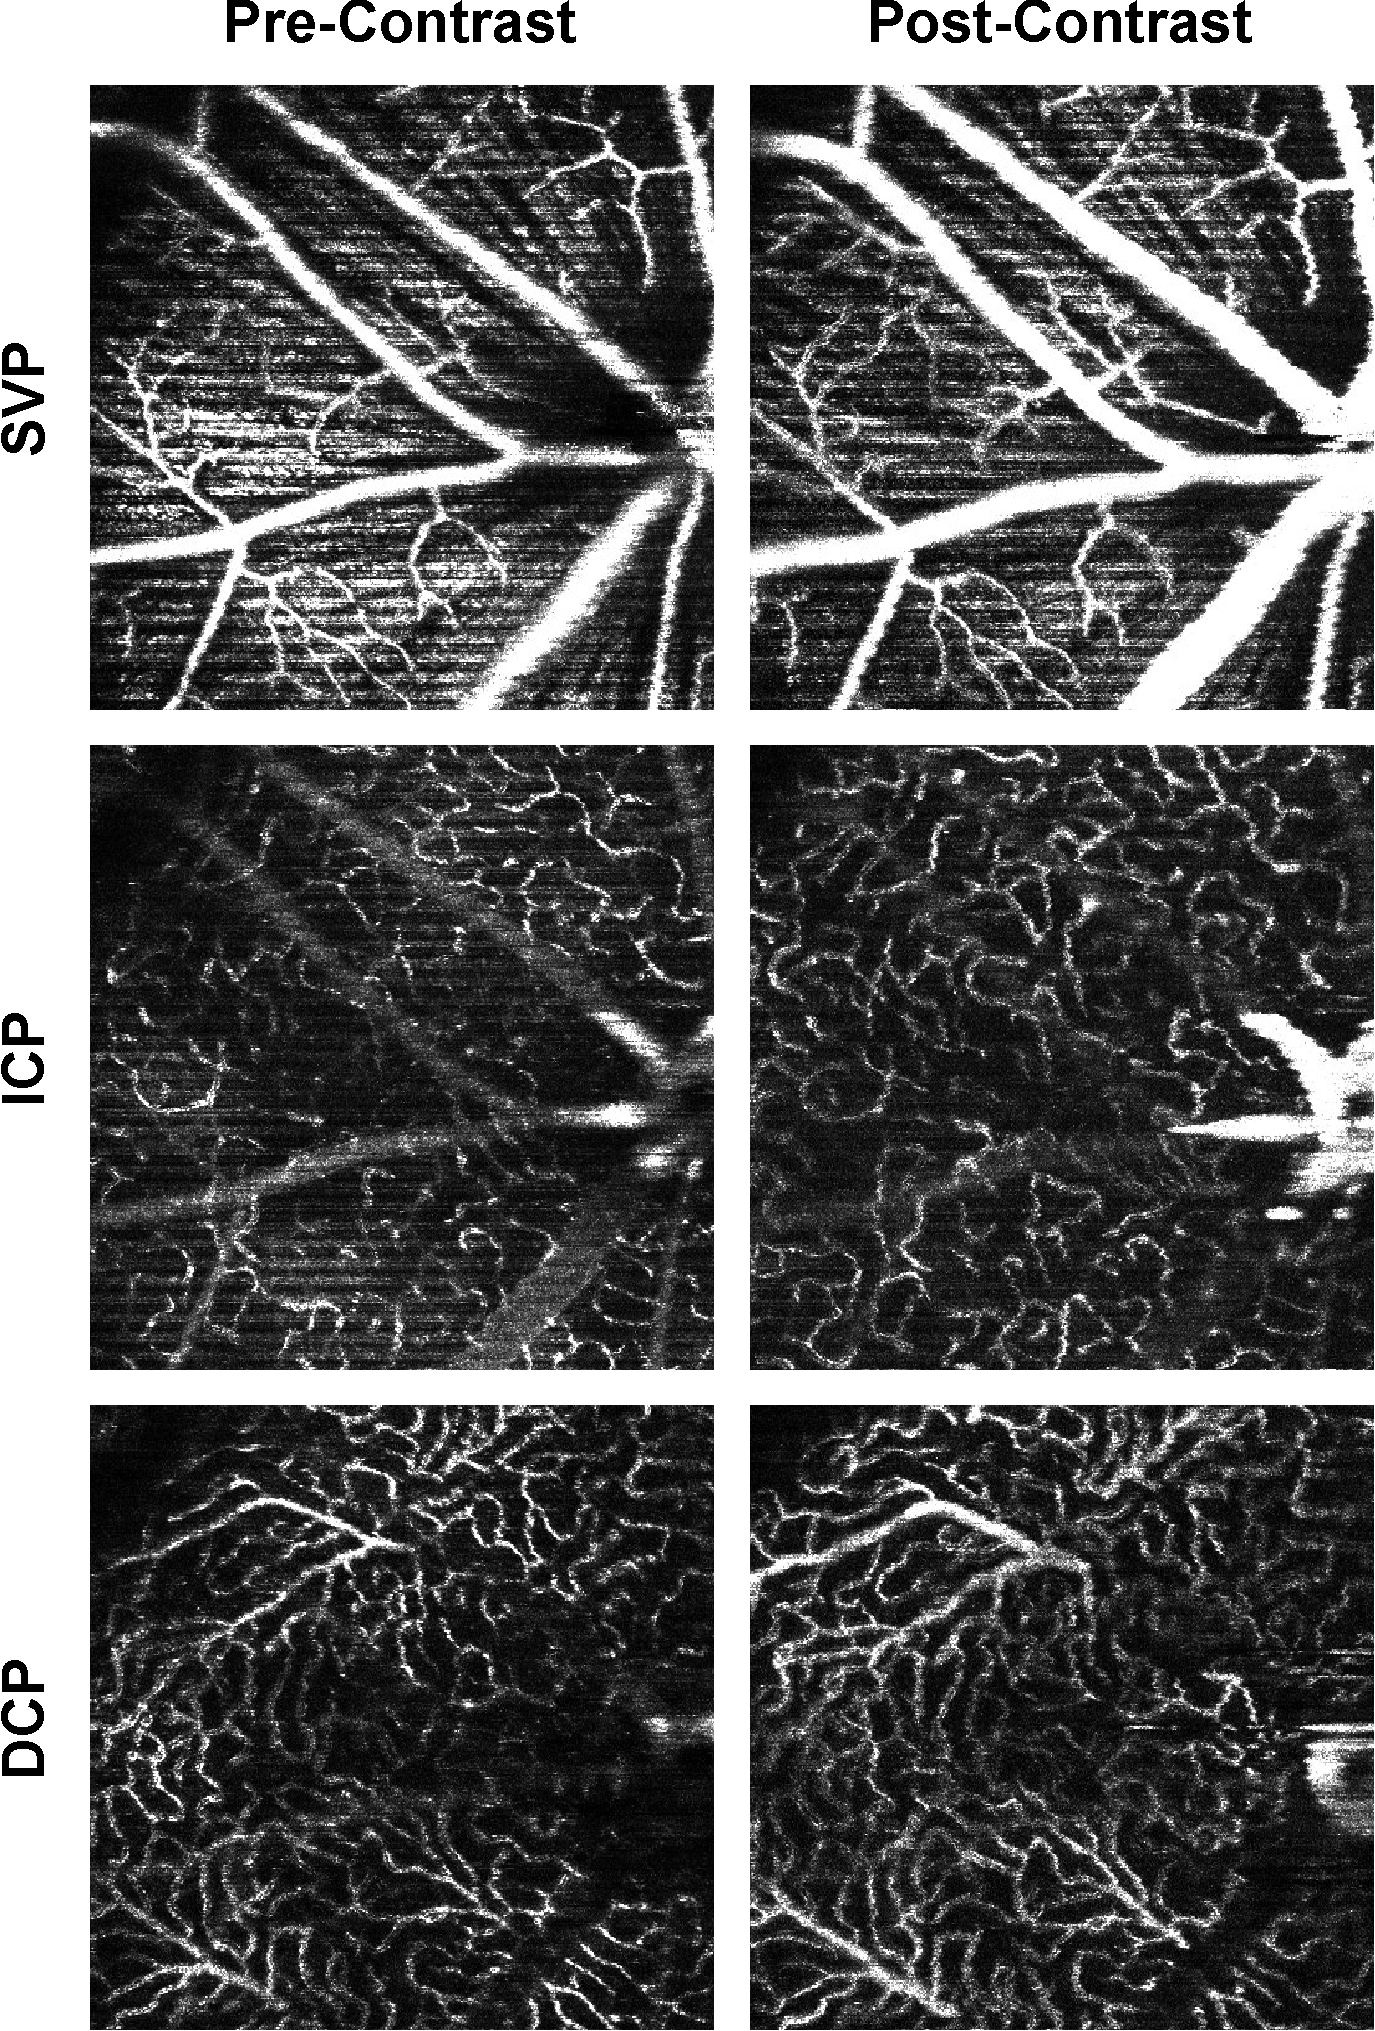
\includegraphics[width=\linewidth,height=\dimexpr\textheight-\pagetotal-3\baselineskip\relax,keepaspectratio]{figures/Figure_1.pdf} 
% height=\dimexpr\textheight-\pagetotal-#\baselineskip\relax = set the figure height to the remaining space on the page, accounting for the current vertical position and leaving room for caption and label.
    % \dimexpr = allow for dynamic calculation of figure height based on the remaining space on the page.
    % -\pagetotal = account for the vertical space already used on the page, ensuring the figure does not exceed the remaining space.
    % -#\baselineskip = leave room for the figure caption and label, which typically require a few lines of text. Adjust the number of baselineskip (#) as needed to ensure the figure fits well without excessive whitespace.
    % \relax = allow the figure to scale down if necessary to fit within the specified height while maintaining aspect ratio.
% \label{fig:enface}
% \end{figure}

\begin{figure}[H] 
\centering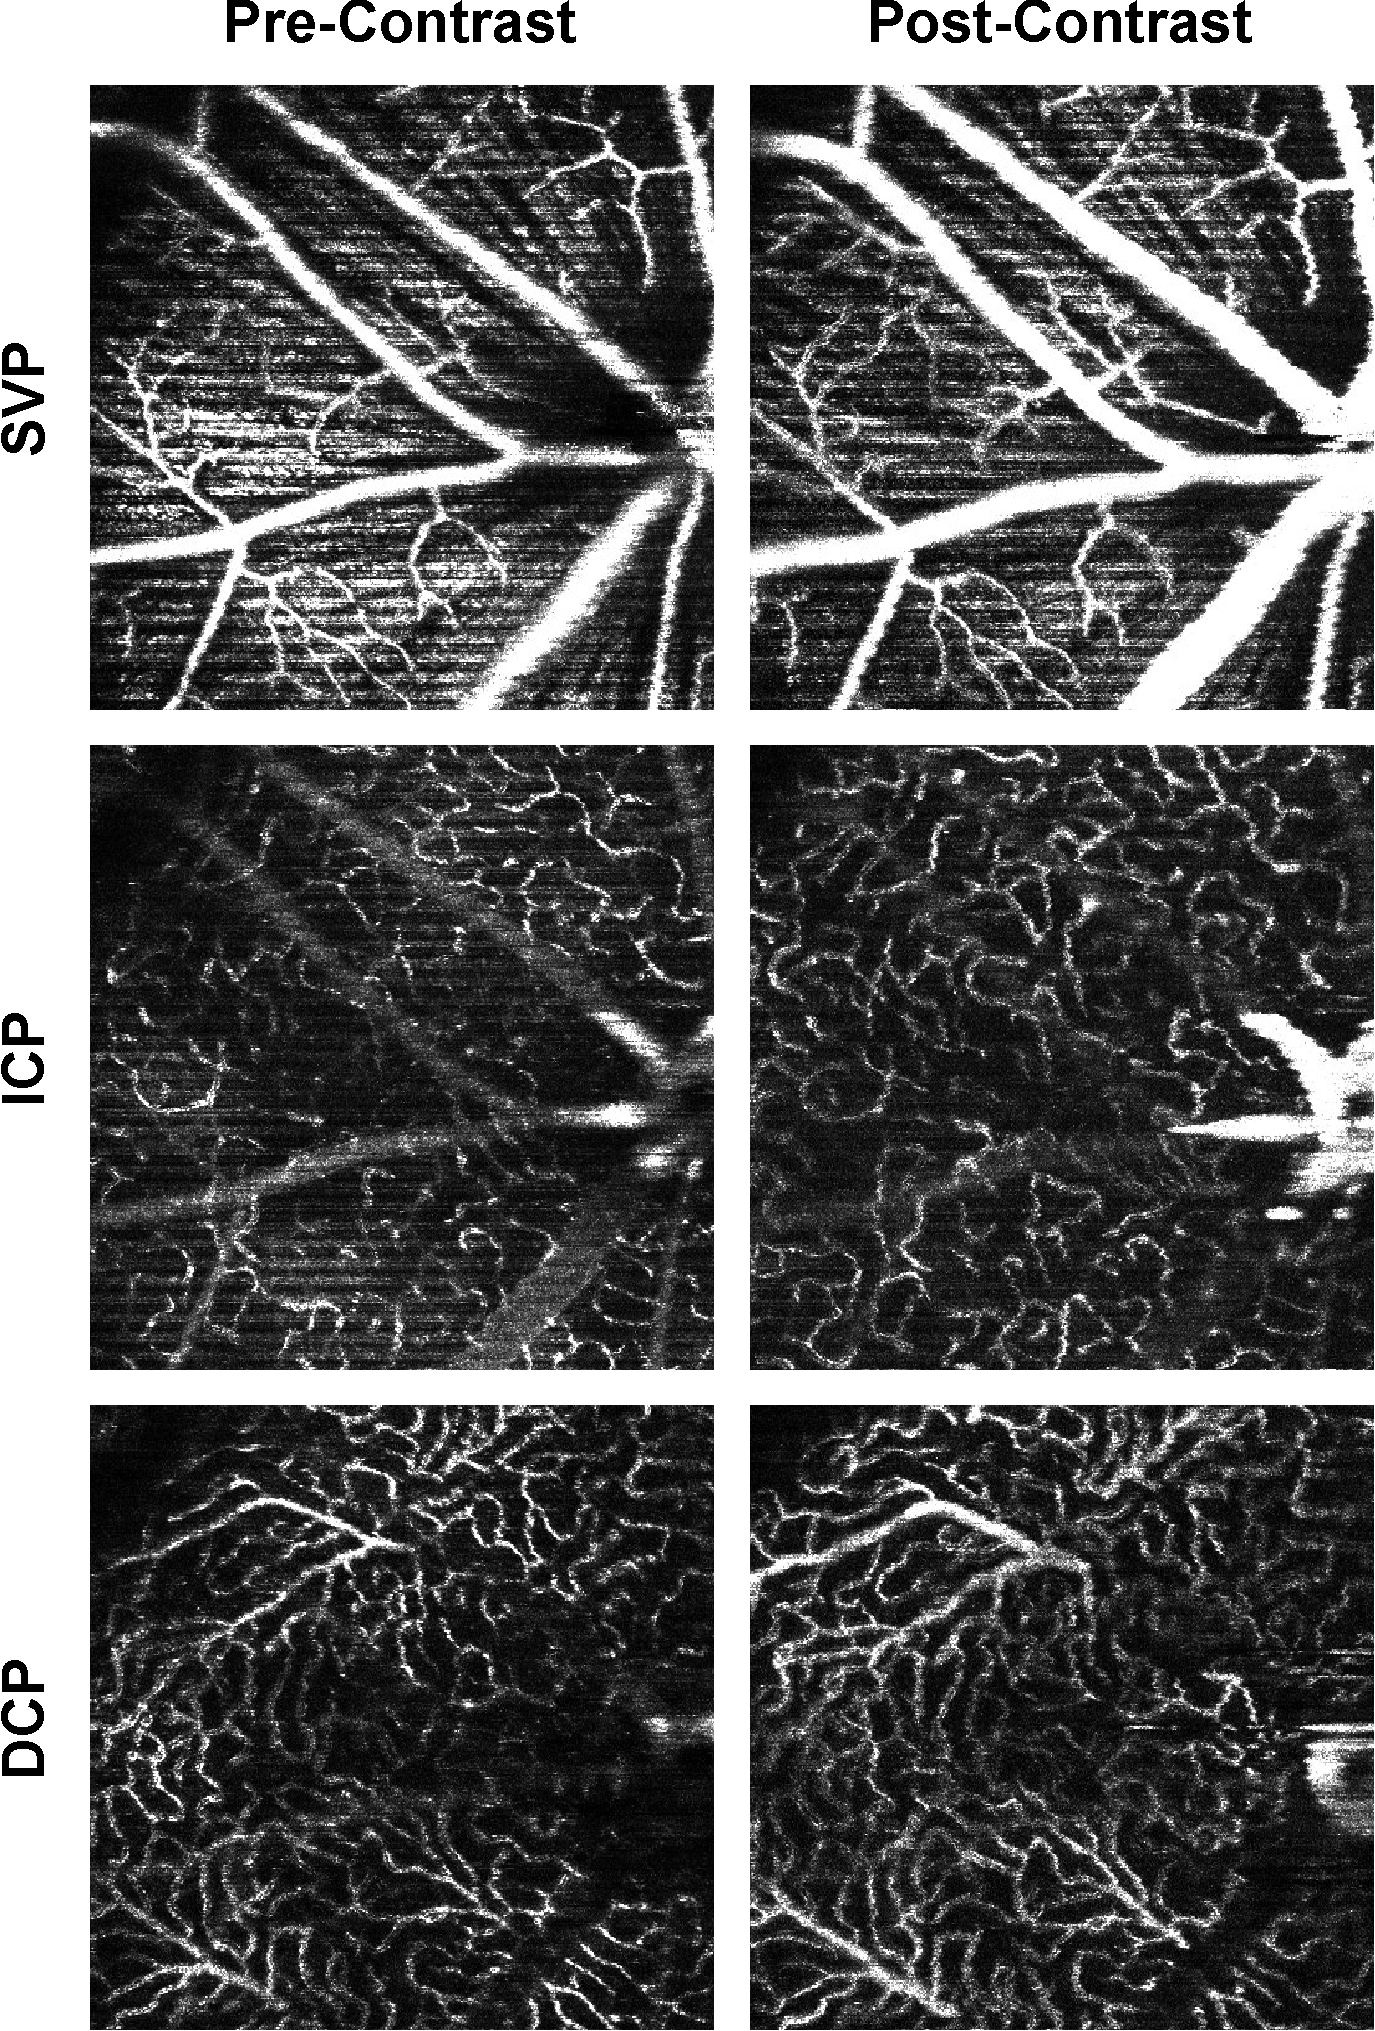
\includegraphics[width=0.45\linewidth,keepaspectratio]{figures/Figure_1.pdf} 
\caption{OCTA MIP en face of the SVP, ICP, and DCP before (left) and after (right) the administration of Intralipid 20\%. Vessels appear visibly wider and brighter post-contrast across all layers, most prominently in the larger vessels.}
\label{fig:enface}
\end{figure}

Figure~\ref{fig:enface} shows OCTA MIP en face of the superficial vascular plexus (SVP), intermediate capillary plexus (ICP), and deep capillary plexus (DCP) before and after contrast injection. Across all three layers, vessels appeared visibly wider and brighter post-contrast injection, consistent with previous literature showing that OCTA underestimates vessel diameter in the absence of a contrast agent~\cite{merkleHighresolutionDepthresolvedVascular2021}. This effect was most pronounced in the larger vessels, especially in the SVP, where the major retinal arteries and veins appeared noticeably thicker after contrast administration. In the ICP and DCP, the capillary networks also showed improved visibility, though the effect was less dramatic.

DyC OCTA projections helped visualise the temporal changes in vessel diameter pre- and post-contrast injection (Fig.~\ref{fig:dycoct}). Pre-contrast injection, the vessel cross-sections appeared narrower than their true diameter (Fig.~\ref{fig:dycoct}a), which could be due to lateral edge signal suppression by the RBC orientation artefact~\cite{bernucciInvestigationArtifactsRetinal2018}.~\textcolor{red}{At peak contrast, the Intralipid filled the vascular lumen uniformly and showed the full extent of the vessel cross-section (Fig.~\ref{fig:dycoct}b). However, the high scattering nature of the contrast agent produced light diffusion beyond the vessel wall, resulting in an apparent vessel diameter that slightly exceeded the true anatomical diameter. In the post-contrast phase, the signal stabilised as the initial bolus cleared, and the vessel boundaries remained more visible than before injection without the overestimation observed at peak contrast (Fig.~\ref{fig:dycoct}c). The MIP and the corresponding binary mask over time (Figs.~\ref{fig:dycoct}d--e) showed the observed temporal changes in vessel diameter across the three phases. The mean OCTA intensity (Fig.~\ref{fig:dycoct}f) showed a sharp increase post-contrast injection, followed by a decrease to a new steady state that remained elevated above the pre-contrast baseline.} These observations confirm that the contrast agent does significantly enhance vessel visibility and diameter, and that the post-contrast images show improved vessel delineation compared to pre-contrast.

\begin{figure}[H]
\centering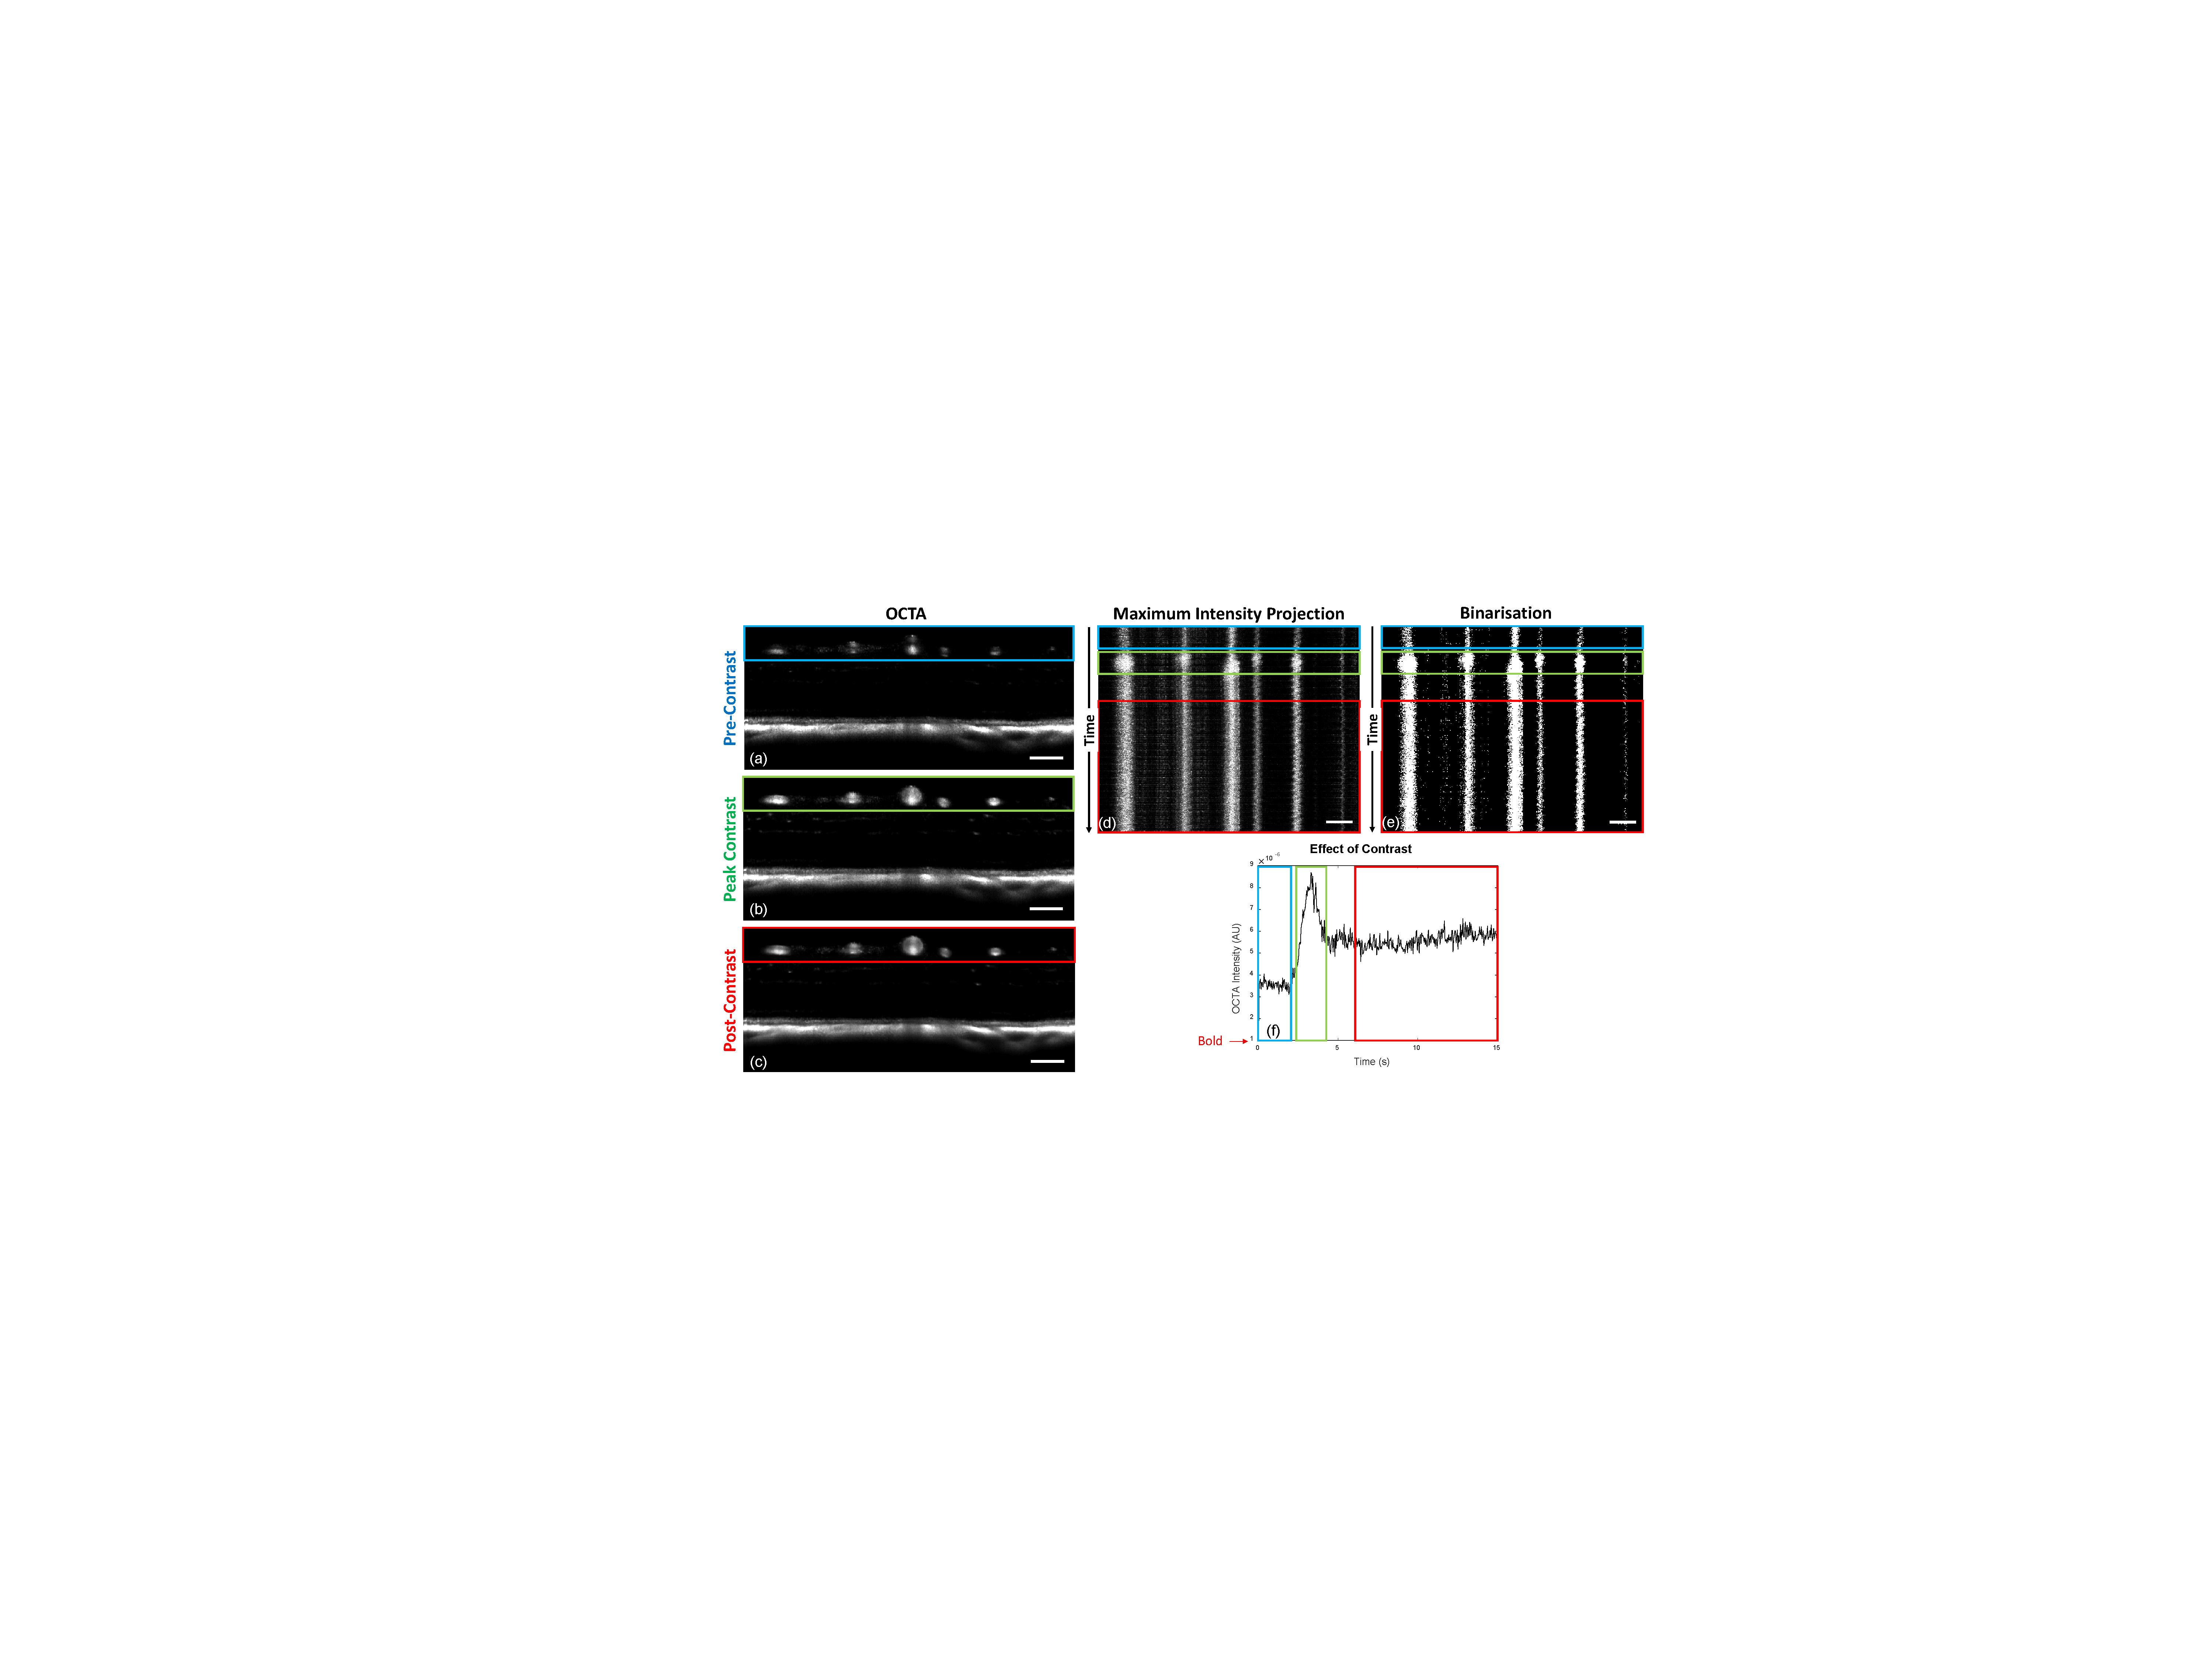
\includegraphics[width=\linewidth,height=\dimexpr\textheight-\pagetotal-8\baselineskip\relax,keepaspectratio]{figures/Figure_2.pdf}
\caption{DyC-OCT B-scan angiograms at (a) pre-contrast, (b) peak contrast, and (c) post-contrast timepoints.~(d) MIP and (e) binarisation of the vessel cross-sections over time, with coloured boxes indicating the pre-contrast (blue), peak-contrast (green), and post-contrast (red) windows.~(f) Mean OCTA intensity over time, showing the temporal intensity dynamics.~\textcolor{red}{All scale bars are 100\,\textmu{}m.}}
\label{fig:dycoct}
\end{figure}

\subsection{Accuracy and linearity of diameter measurements}
\label{subsec:linearity_accuracy_model}
To evaluate the accuracy and linearity of all diameter measurement approaches, the calculated diameter values were plotted against the ground truth for each vessel across three conditions: pre-contrast, peak contrast, and post-contrast. A linear regression was fitted to each condition, yielding the slope ($m$) and coefficient of determination ($R^2$), which are summarised in Table~\ref{tab:accuracy_linearity}. A slope of $m = 1$ (black line) indicated perfect agreement with the ground truth, and $R^2$ quantified the goodness of fit of the linear model. For the model-based methods, six combinations were evaluated: two projection methods (MIP and MeIP) by three width metrics ($w_{1/e^2,\,\mathrm{G}}$, $\mathrm{FWHM}_{\mathrm{GG}}$, and $w_{1/e^2,\,\mathrm{GG}}$; Fig.~\ref{fig:scatter_model}). For the binarisation-based methods, diameter was measured at five threshold levels (BW-1 through BW-5) for both MIP (Fig.~\ref{fig:scatter_bw_mip}) and MeIP (Fig.~\ref{fig:scatter_bw_meip}). 

\begin{figure}[H]
\centering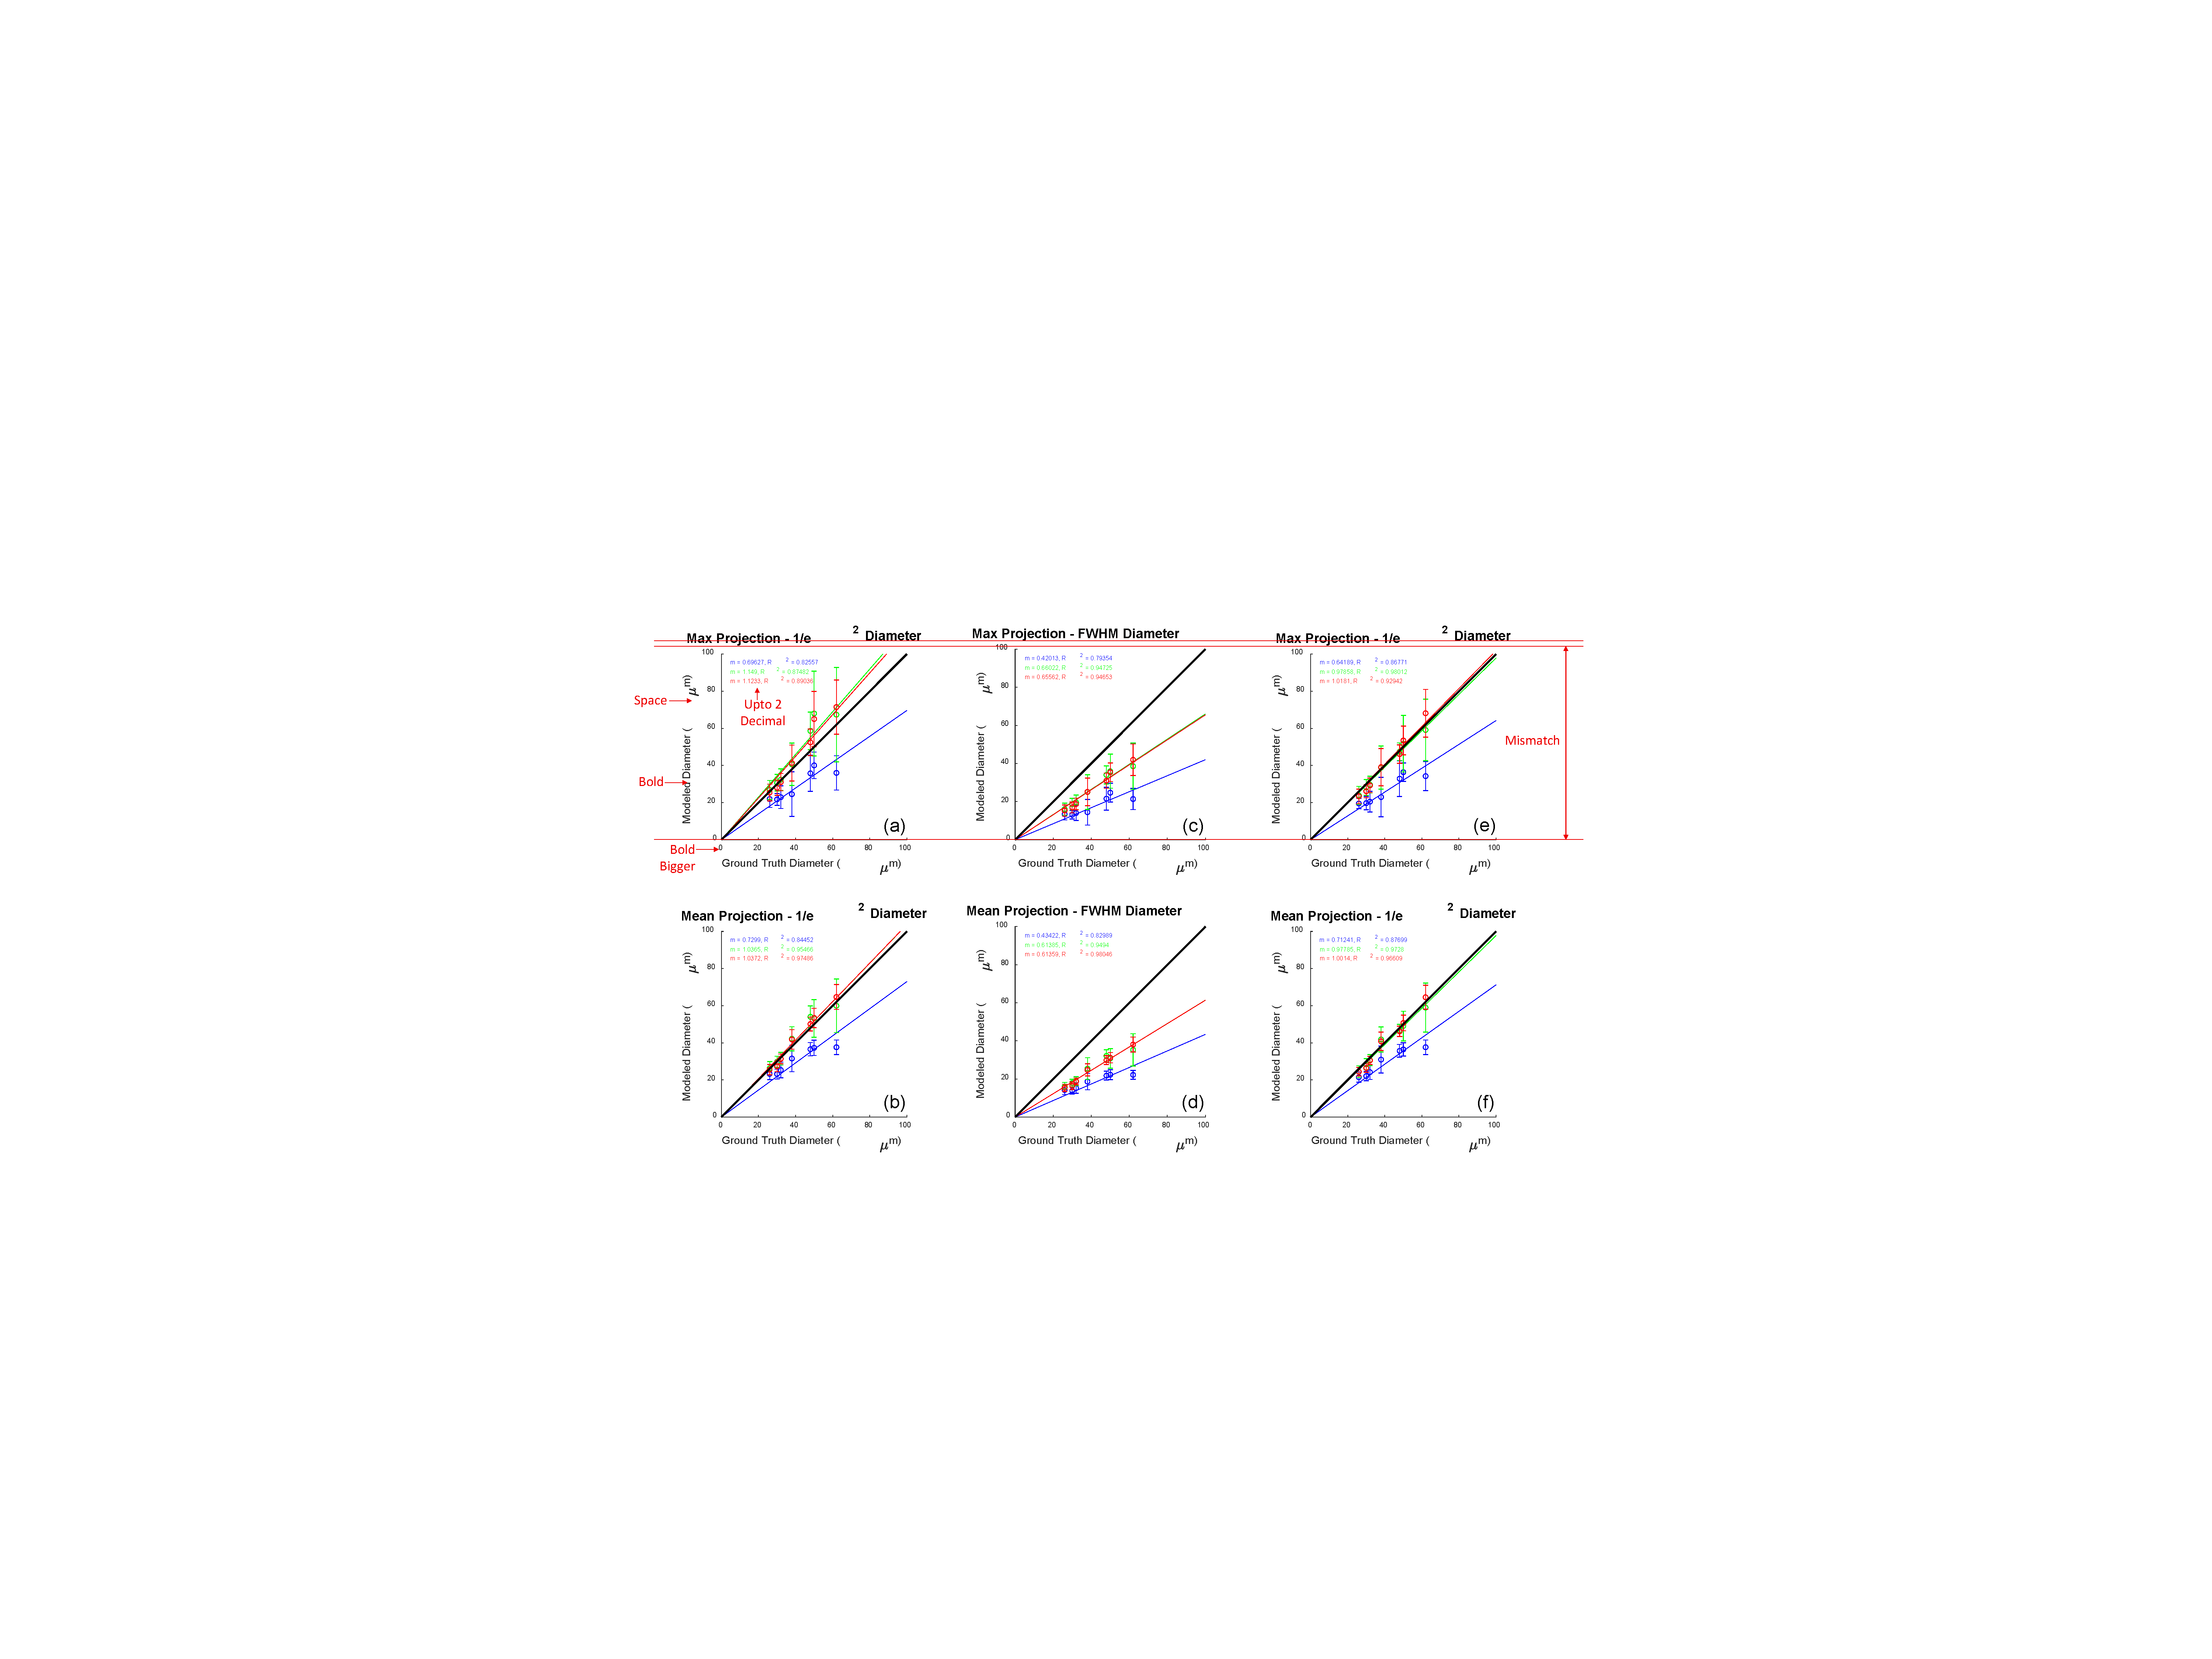
\includegraphics[width=\linewidth,height=\dimexpr\textheight-\pagetotal-8\baselineskip\relax,keepaspectratio]{figures/Figure_4.pdf}
\caption{Modelled versus ground truth vessel diameter using MIP (top row) and MeIP (bottom row). Columns correspond to (a,b) Gaussian $1/e^2$ width, (c,d) GG FWHM, and (e,f) GG $1/e^2$ width. Regression lines and statistics are shown for pre-contrast (blue), peak contrast (green), and post-contrast (red) conditions. The black line indicates the identity line ($m = 1$).}
\label{fig:scatter_model}
\end{figure}

All model-based methods underestimated vessel diameter in pre-contrast data, with slopes ranging from 0.42 to 0.73 (Table~\ref{tab:accuracy_linearity}). Contrast enhancement improved accuracy across all metrics, though the degree of improvement varied. The $\mathrm{FWHM}_{\mathrm{GG}}$ metric remained well below unity even post-contrast. The $w_{1/e^2,\,\mathrm{G}}$ with MIP slightly overestimated post-contrast ($m = 1.12$--$1.15$), while MeIP yielded values closer to unity ($m = 1.04$). The $w_{1/e^2,\,\mathrm{GG}}$ with MeIP provided the best overall agreement, achieving a slope closest to unity with $m = 1.001$ ($R^2 = 0.97$) post-contrast, which was the closest to the identity line of all tested model-based methods. Across all metrics, MeIP mostly outperformed MIP in both accuracy and linearity (Table~\ref{tab:accuracy_linearity}, Fig.~\ref{fig:scatter_model}).

\begin{figure}[htbp]
\centering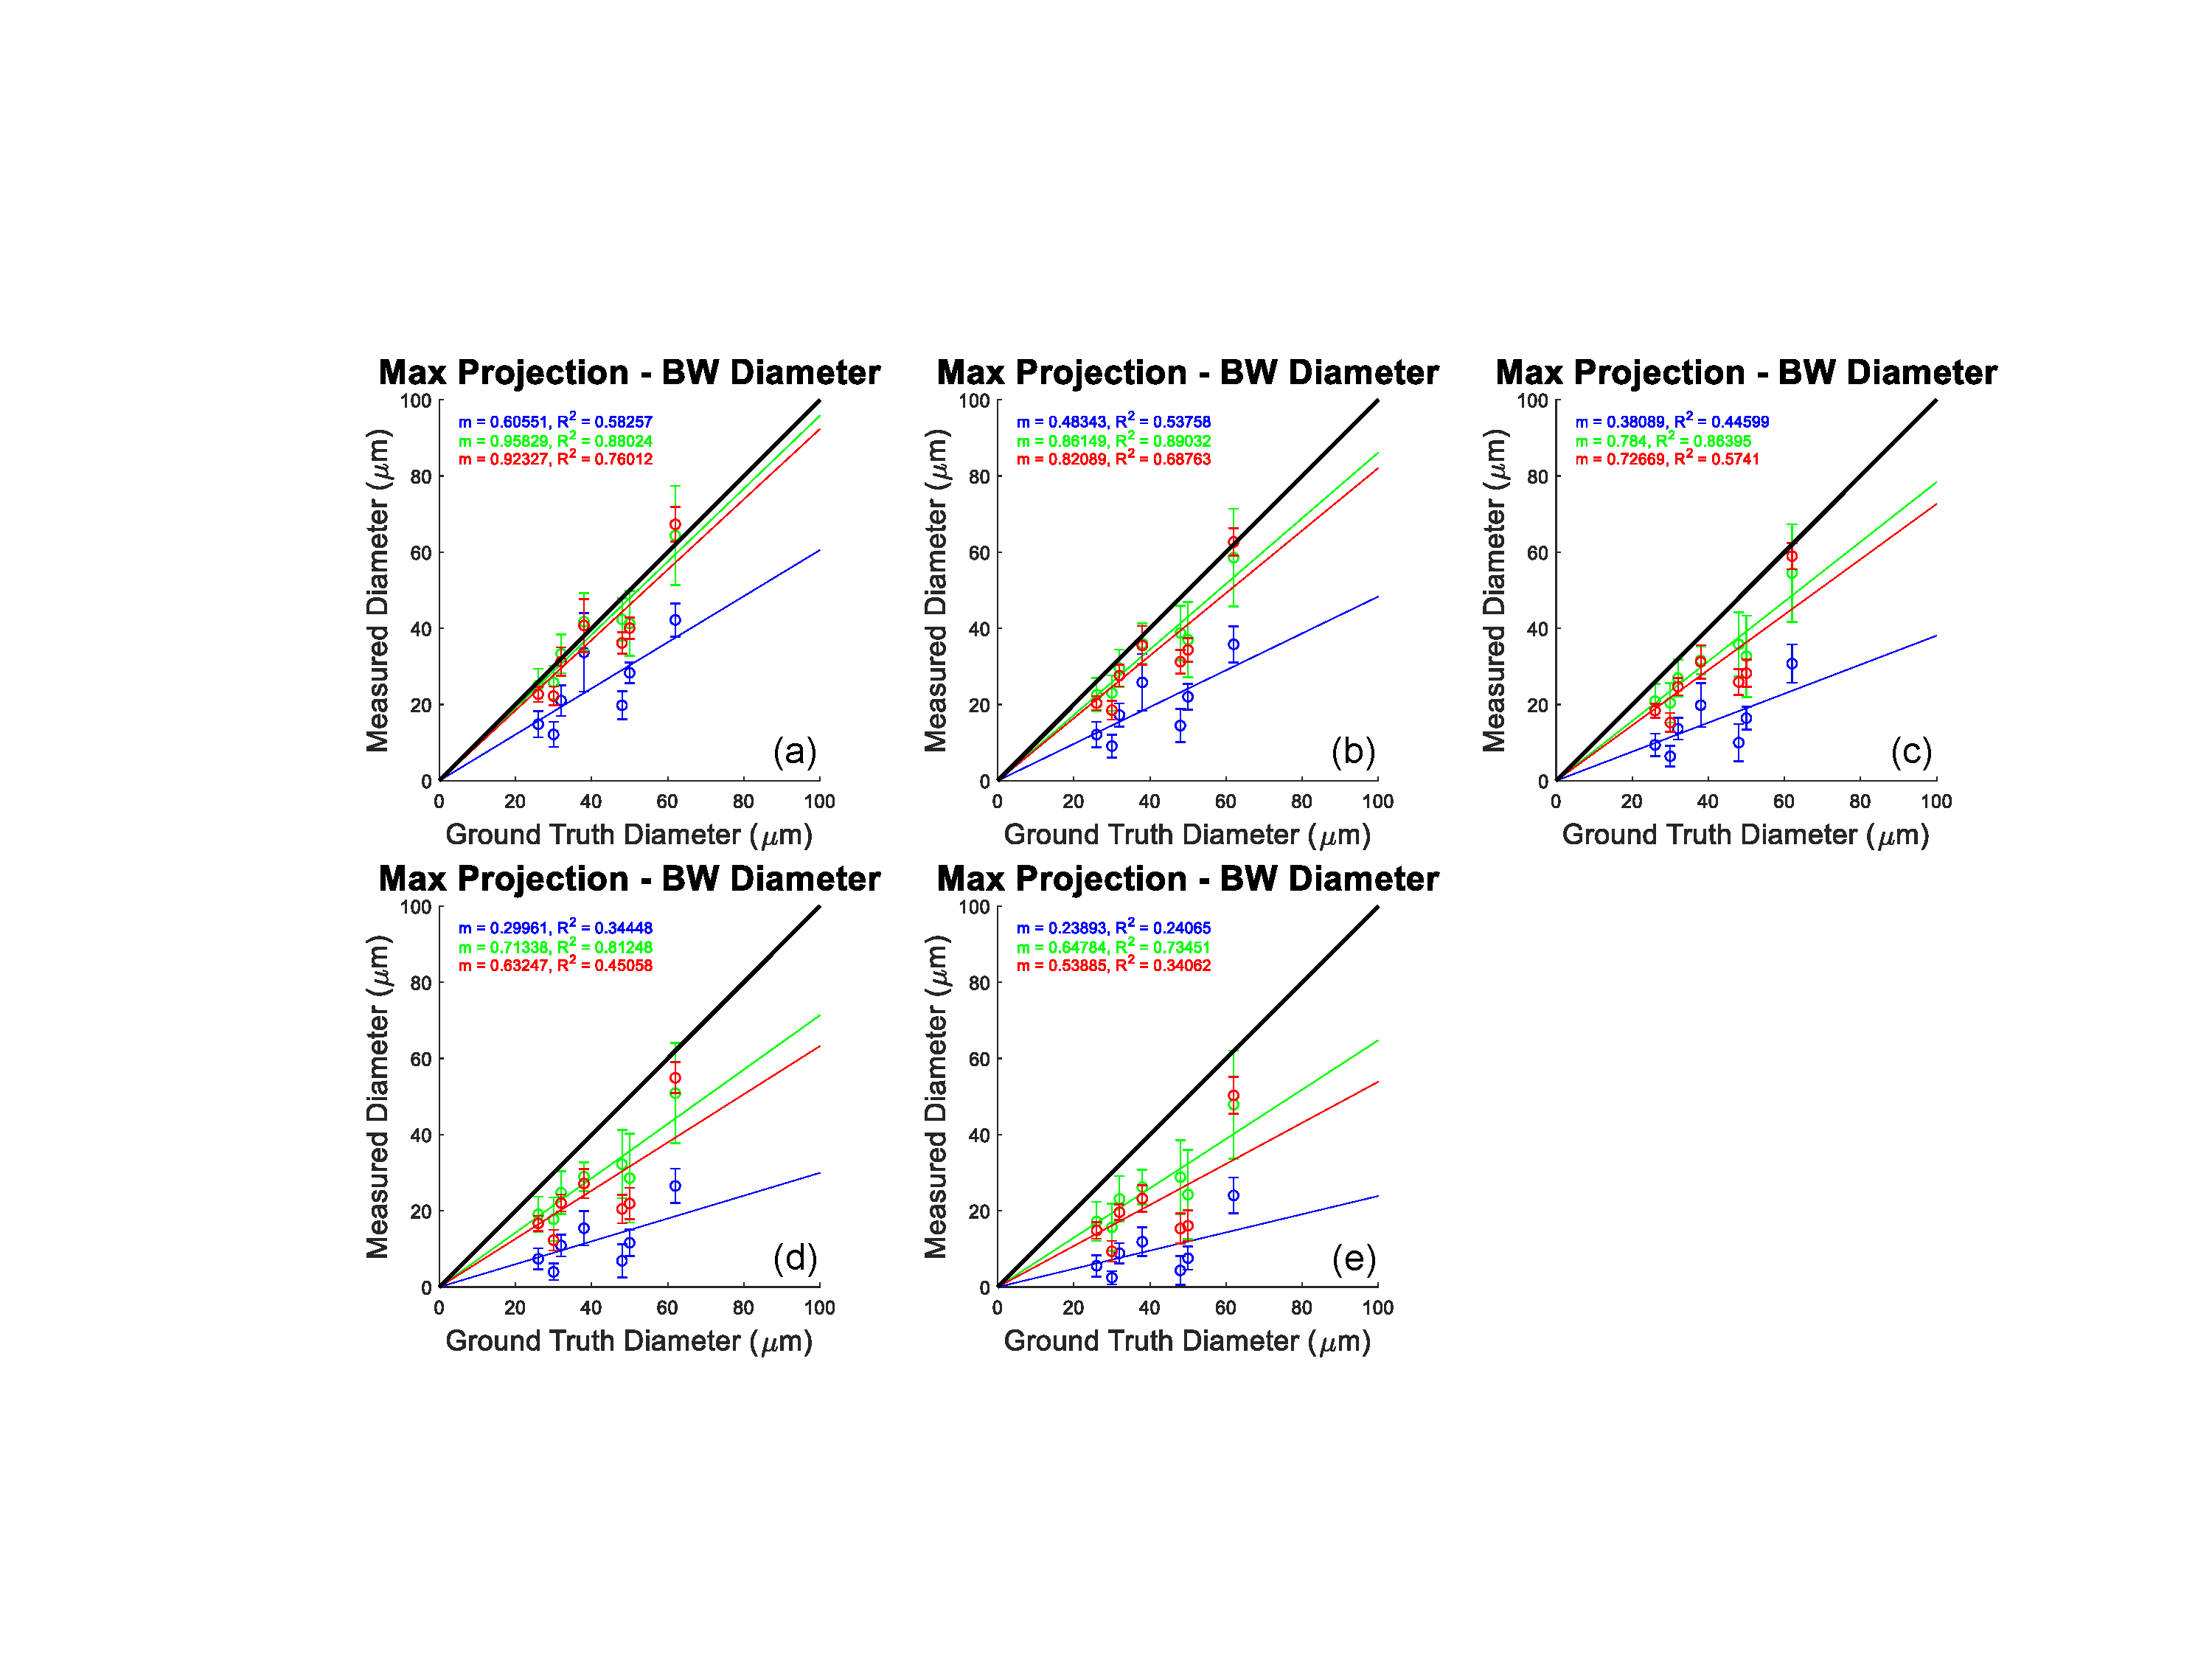
\includegraphics[width=\linewidth,keepaspectratio]{figures/Figure_5.pdf}
\caption{Vessel diameter measured from BW images versus ground truth for MIP at five threshold levels: (a) BW-1 through (e) BW-5. Regression lines and statistics are shown for pre-contrast (blue), peak contrast (green), and post-contrast (red). Both slope $m$ and $R^2$ decrease with increasing threshold values.}
\label{fig:scatter_bw_mip}
\end{figure}

\begin{figure}[htbp]
\centering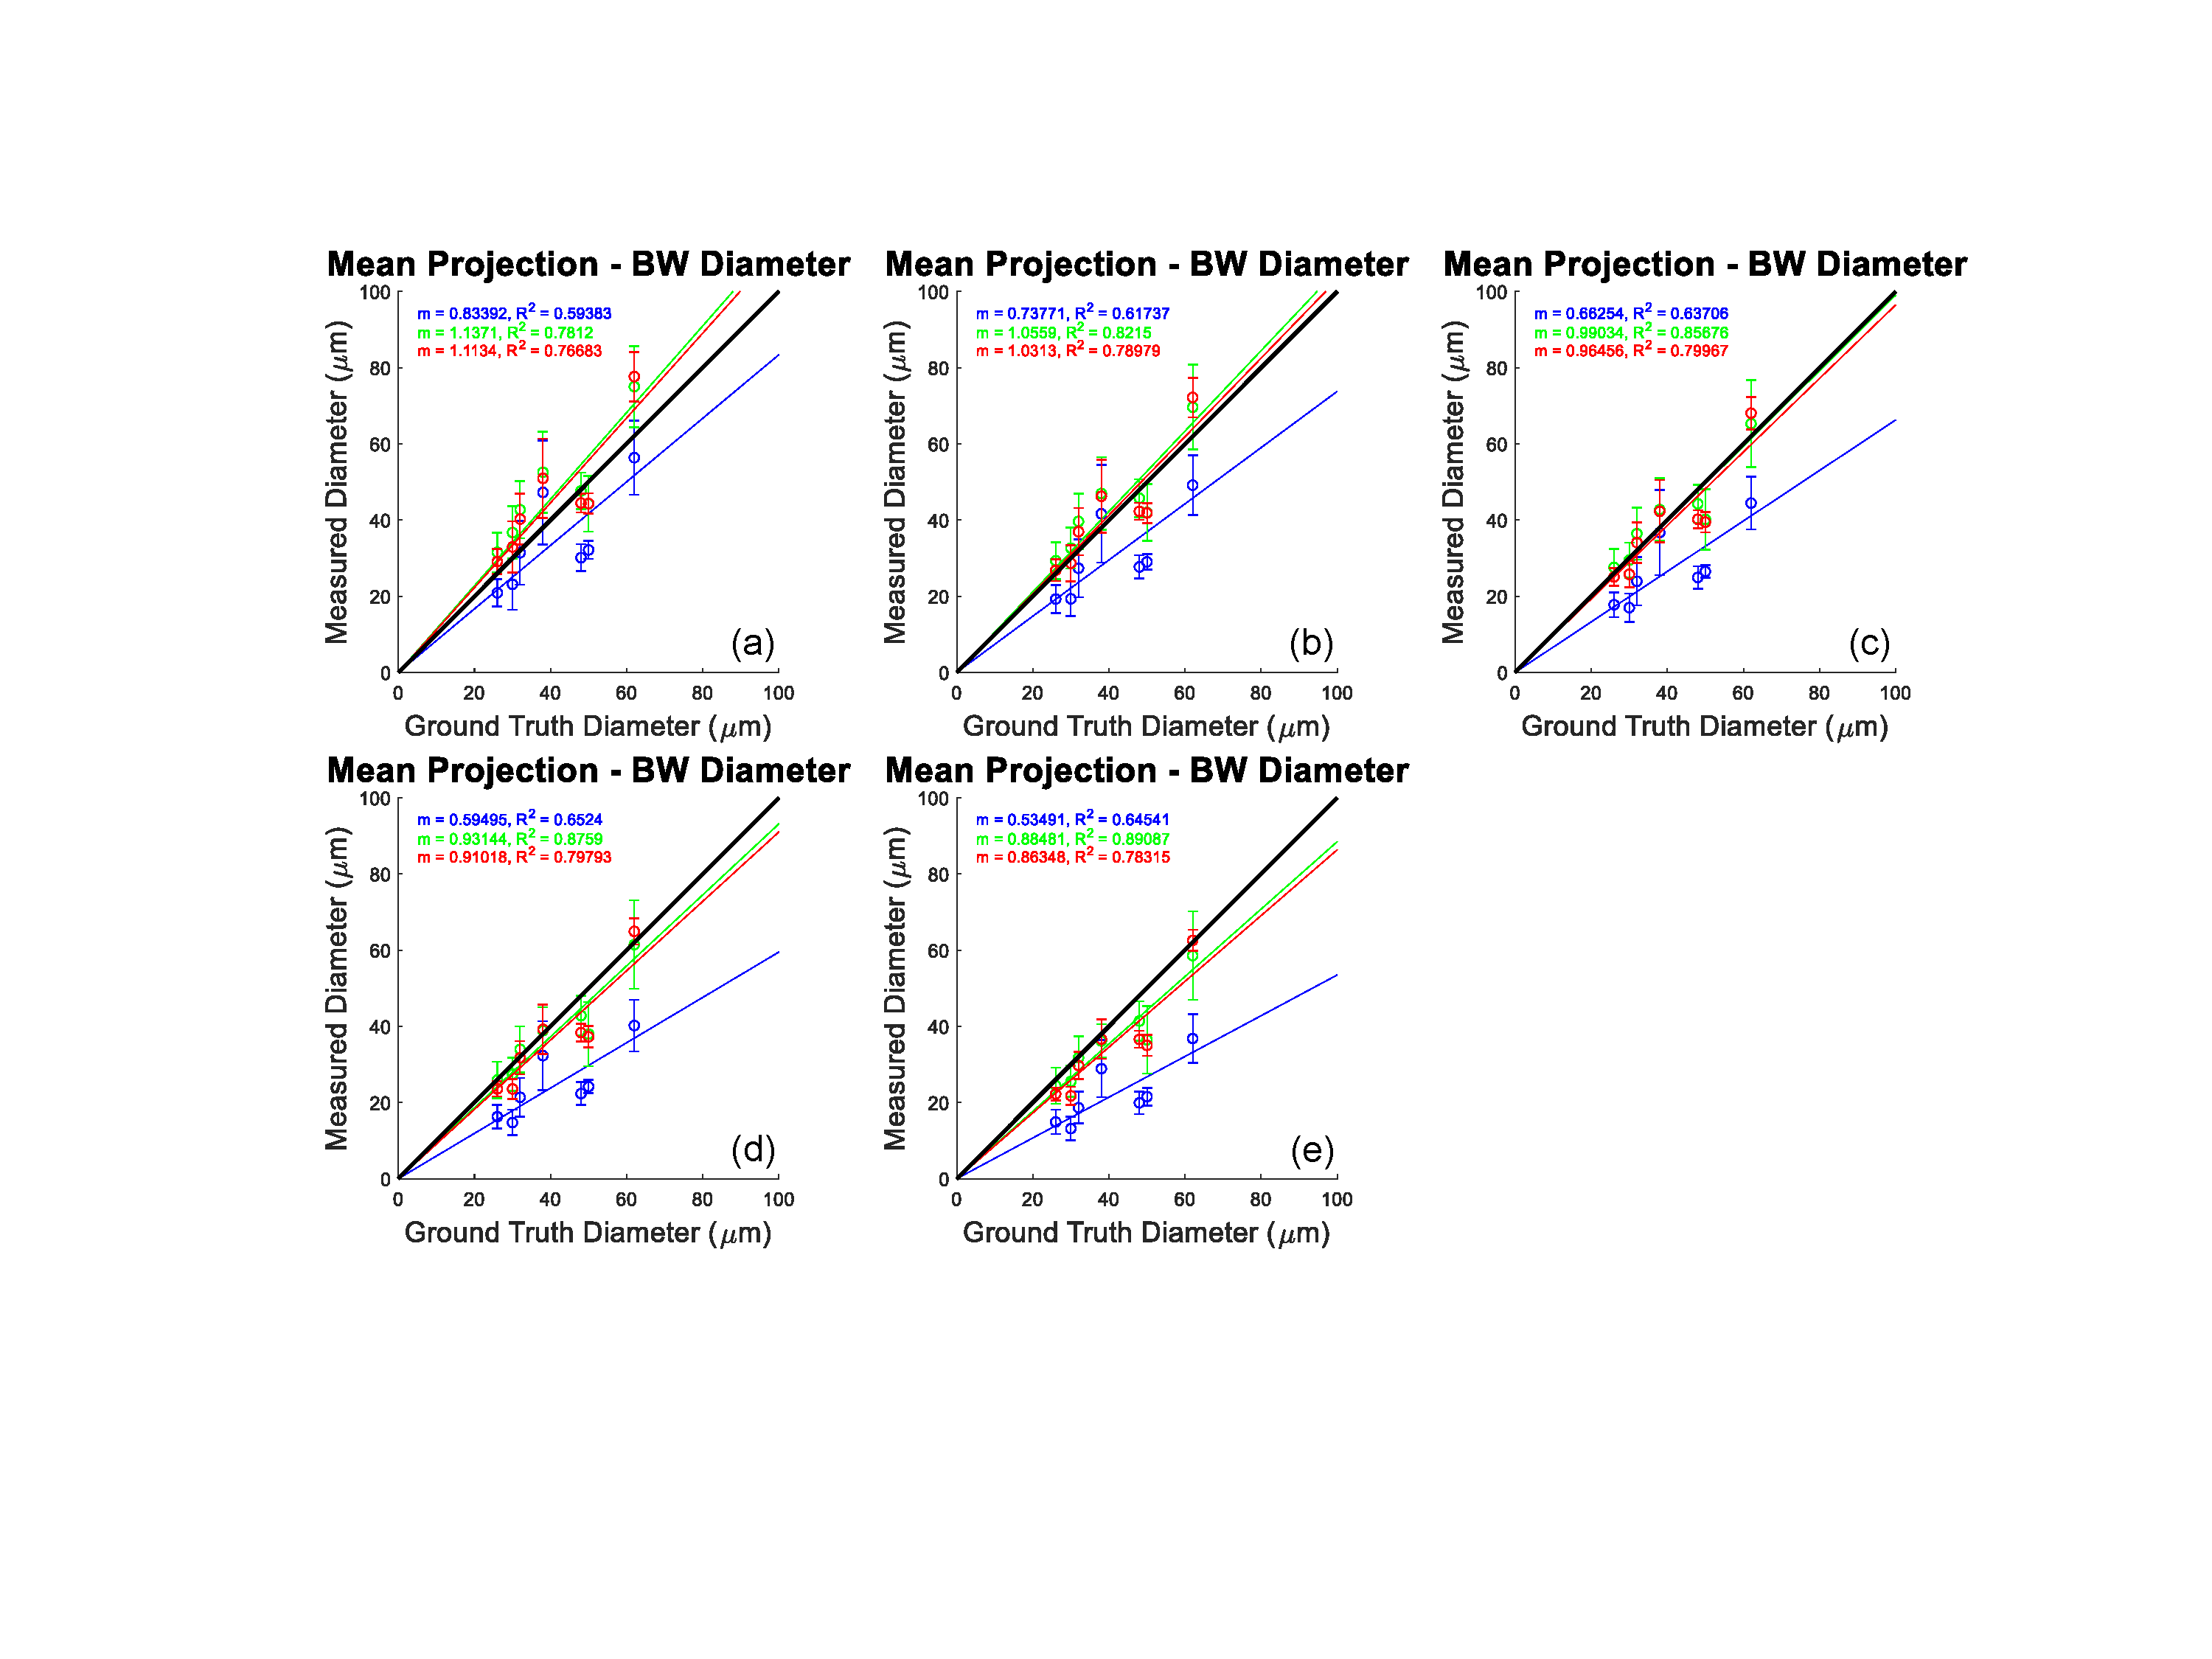
\includegraphics[width=\linewidth,keepaspectratio]{figures/Figure_6.pdf}
\caption{Vessel diameter measured from BW images versus ground truth for MeIP at five threshold levels: (a) BW-1 through (e) BW-5. Regression lines and statistics are shown for pre-contrast (blue), peak contrast (green), and post-contrast (red) conditions. MeIP yielded higher slopes and more stable $R^2$ values compared to MIP (Fig.~\ref{fig:scatter_bw_mip}).}
\label{fig:scatter_bw_meip}
\end{figure}

For binarisation-based methods, the slope decreased with increase in threshold values across all contrast conditions and projections (Table~\ref{tab:accuracy_linearity}). MeIP $m$ values were consistently higher than MIP across all threshold and contrast conditions. Also, across all contrast conditions, $m$ dropped more significantly with increase in threshold for MIP than for MeIP. For MIP, the pre- and post-contrast $R^2$ decreased substantially with increase in threshold, whereas for MeIP, the $R^2$ remained relatively stable. At lower threshold values and at peak and post-contrast, MeIP overestimated the vessel diameter more than MIP. At peak and post-contrast, MeIP BW-3 achieved a slope of $m = 0.99$ and $m = 0.97$ respectively, though with a lower $R^2 = 0.86$ and $R^2 = 0.80$ respectively, compared to $w_{1/e^2,\,\mathrm{GG}}$ which achieved $m = 1.001$ with a higher $R^2 = 0.97$. Overall, MeIP provided more reliable binarisation-based diameter measurements than MIP.

\begin{table}[htbp]
\caption{Summary of slope ($m$) and coefficient of determination ($R^2$) for all diameter measurement methods across pre-contrast, peak contrast, and post-contrast conditions. Methods are grouped as binarisation-based and model-based. Bold slope values indicate agreement within 10\% of unity ($0.9 \leq m \leq 1.1$).}
\label{tab:accuracy_linearity}
\centering
\resizebox{\textwidth}{!}{%
\begin{tabular}{l c c | c c | c c | c c | c c || c c | c c | c c}
\hline
 & \multicolumn{2}{c|}{\textbf{BW-1}} & \multicolumn{2}{c|}{\textbf{BW-2}} & \multicolumn{2}{c|}{\textbf{BW-3}} & \multicolumn{2}{c|}{\textbf{BW-4}} & \multicolumn{2}{c||}{\textbf{BW-5}} & \multicolumn{2}{c|}{\textbf{$w_{1/e^2,\,\mathrm{G}}$}} & \multicolumn{2}{c|}{\textbf{$\mathrm{FWHM}_{\mathrm{GG}}$}} & \multicolumn{2}{c}{\textbf{$w_{1/e^2,\,\mathrm{GG}}$}} \\
 & MIP & MeIP & MIP & MeIP & MIP & MeIP & MIP & MeIP & MIP & MeIP & MIP & MeIP & MIP & MeIP & MIP & MeIP \\
\hline
\multicolumn{17}{l}{\textit{Slope ($m$)}} \\
\hline
Pre  & 0.61 & 0.83 & 0.48 & 0.74 & 0.38 & 0.66 & 0.30 & 0.59 & 0.24 & 0.53 & 0.70 & 0.73 & 0.42 & 0.43 & 0.64 & 0.71 \\
Peak & \textbf{0.96} & 1.14 & 0.86 & \textbf{1.06} & 0.78 & \textbf{0.99} & 0.71 & \textbf{0.93} & 0.65 & 0.88 & 1.15 & \textbf{1.04} & 0.66 & 0.61 & \textbf{0.98} & \textbf{0.98} \\
Post & \textbf{0.92} & 1.11 & 0.82 & \textbf{1.03} & 0.73 & \textbf{0.97} & 0.63 & \textbf{0.91} & 0.54 & 0.86 & 1.12 & \textbf{1.04} & 0.66 & 0.61 & \textbf{1.02} & \textbf{1.00} \\
\hline
\multicolumn{17}{l}{\textit{Coefficient of determination ($R^2$)}} \\
\hline
Pre  & 0.58 & 0.59 & 0.54 & 0.62 & 0.45 & 0.64 & 0.34 & 0.65 & 0.24 & 0.65 & 0.83 & 0.84 & 0.79 & 0.83 & 0.87 & 0.88 \\
Peak & 0.88 & 0.78 & 0.89 & 0.82 & 0.86 & 0.86 & 0.81 & 0.88 & 0.74 & 0.89 & 0.87 & 0.95 & 0.95 & 0.95 & 0.98 & 0.97 \\
Post & 0.76 & 0.77 & 0.69 & 0.79 & 0.57 & 0.80 & 0.45 & 0.80 & 0.34 & 0.78 & 0.89 & 0.97 & 0.95 & 0.98 & 0.93 & 0.97 \\
\hline
\end{tabular}%
}
\end{table}

\subsection{Repeatability and linearity comparison across all methods}
\label{subsec:comparison_all_methods}
\textcolor{red}{(confirm the values reported here with the actual data, as these are just extracted from the bar plots.)}

To compare the repeatability and linearity across BW1--5 and the model based approach, the coefficient of variation (CoV) and $R^2$ were computed (Fig.~\ref{fig:cov_r2}). For MIP based measurements (Fig.~\ref{fig:cov_r2}a), the CoV of BW method increased with increase in threshold while the CoV of the model based methods remained relatively stable. With increase in threshold values BW1--5, the CoV increased from approximately 0.2 to 0.47 for pre-contrast, 0.17 to 0.32 for peak contrast, and 0.1 to 0.18 for post-contrast data. The model based methods (G-$e^2$, GG-HM, GG-$e^2$) exhibited CoV values of approximately 0.24--0.27 for pre-contrast data, with reduced values of approximately 0.16--0.18 post-contrast. For MeIP based measurements (Fig.~\ref{fig:cov_r2}b), the BW CoV values were lower and more stable across thresholds, with values observed as approximately 0.18--0.20 pre-contrast, 0.16--0.17 peak contrast, and 0.09--0.13 post-contrast. The model based CoV values were lower as well, with values observed as approximately 0.13--0.15 pre-contrast, increasing slightly to 0.13--0.16, and then decreasing to approximately 0.09--0.10 post-contrast.

The linearity results followed a complementary pattern. For MIP (Fig.~\ref{fig:cov_r2}c), the BW $R^2$ values declined sharply from approximately 0.59 at BW-1 to 0.23 at BW-5 for pre-contrast data, while the model based $R^2$ values ranged from 0.80 to 0.86 pre-contrast and reached 0.90--0.97 at peak and post-contrast. For MeIP (Fig.~\ref{fig:cov_r2}d), the BW $R^2$ values were more stable (approximately 0.60--0.65 pre-contrast) but still substantially lower than the model based values (0.83--0.85 pre-contrast, reaching 0.95--0.98 post-contrast). Taken together, these results demonstrate that model based methods consistently outperformed binarisation in both repeatability and linearity across all contrast conditions, and that MeIP based processing yielded superior performance compared with MIP for both method categories.

\begin{figure}[H]
\centering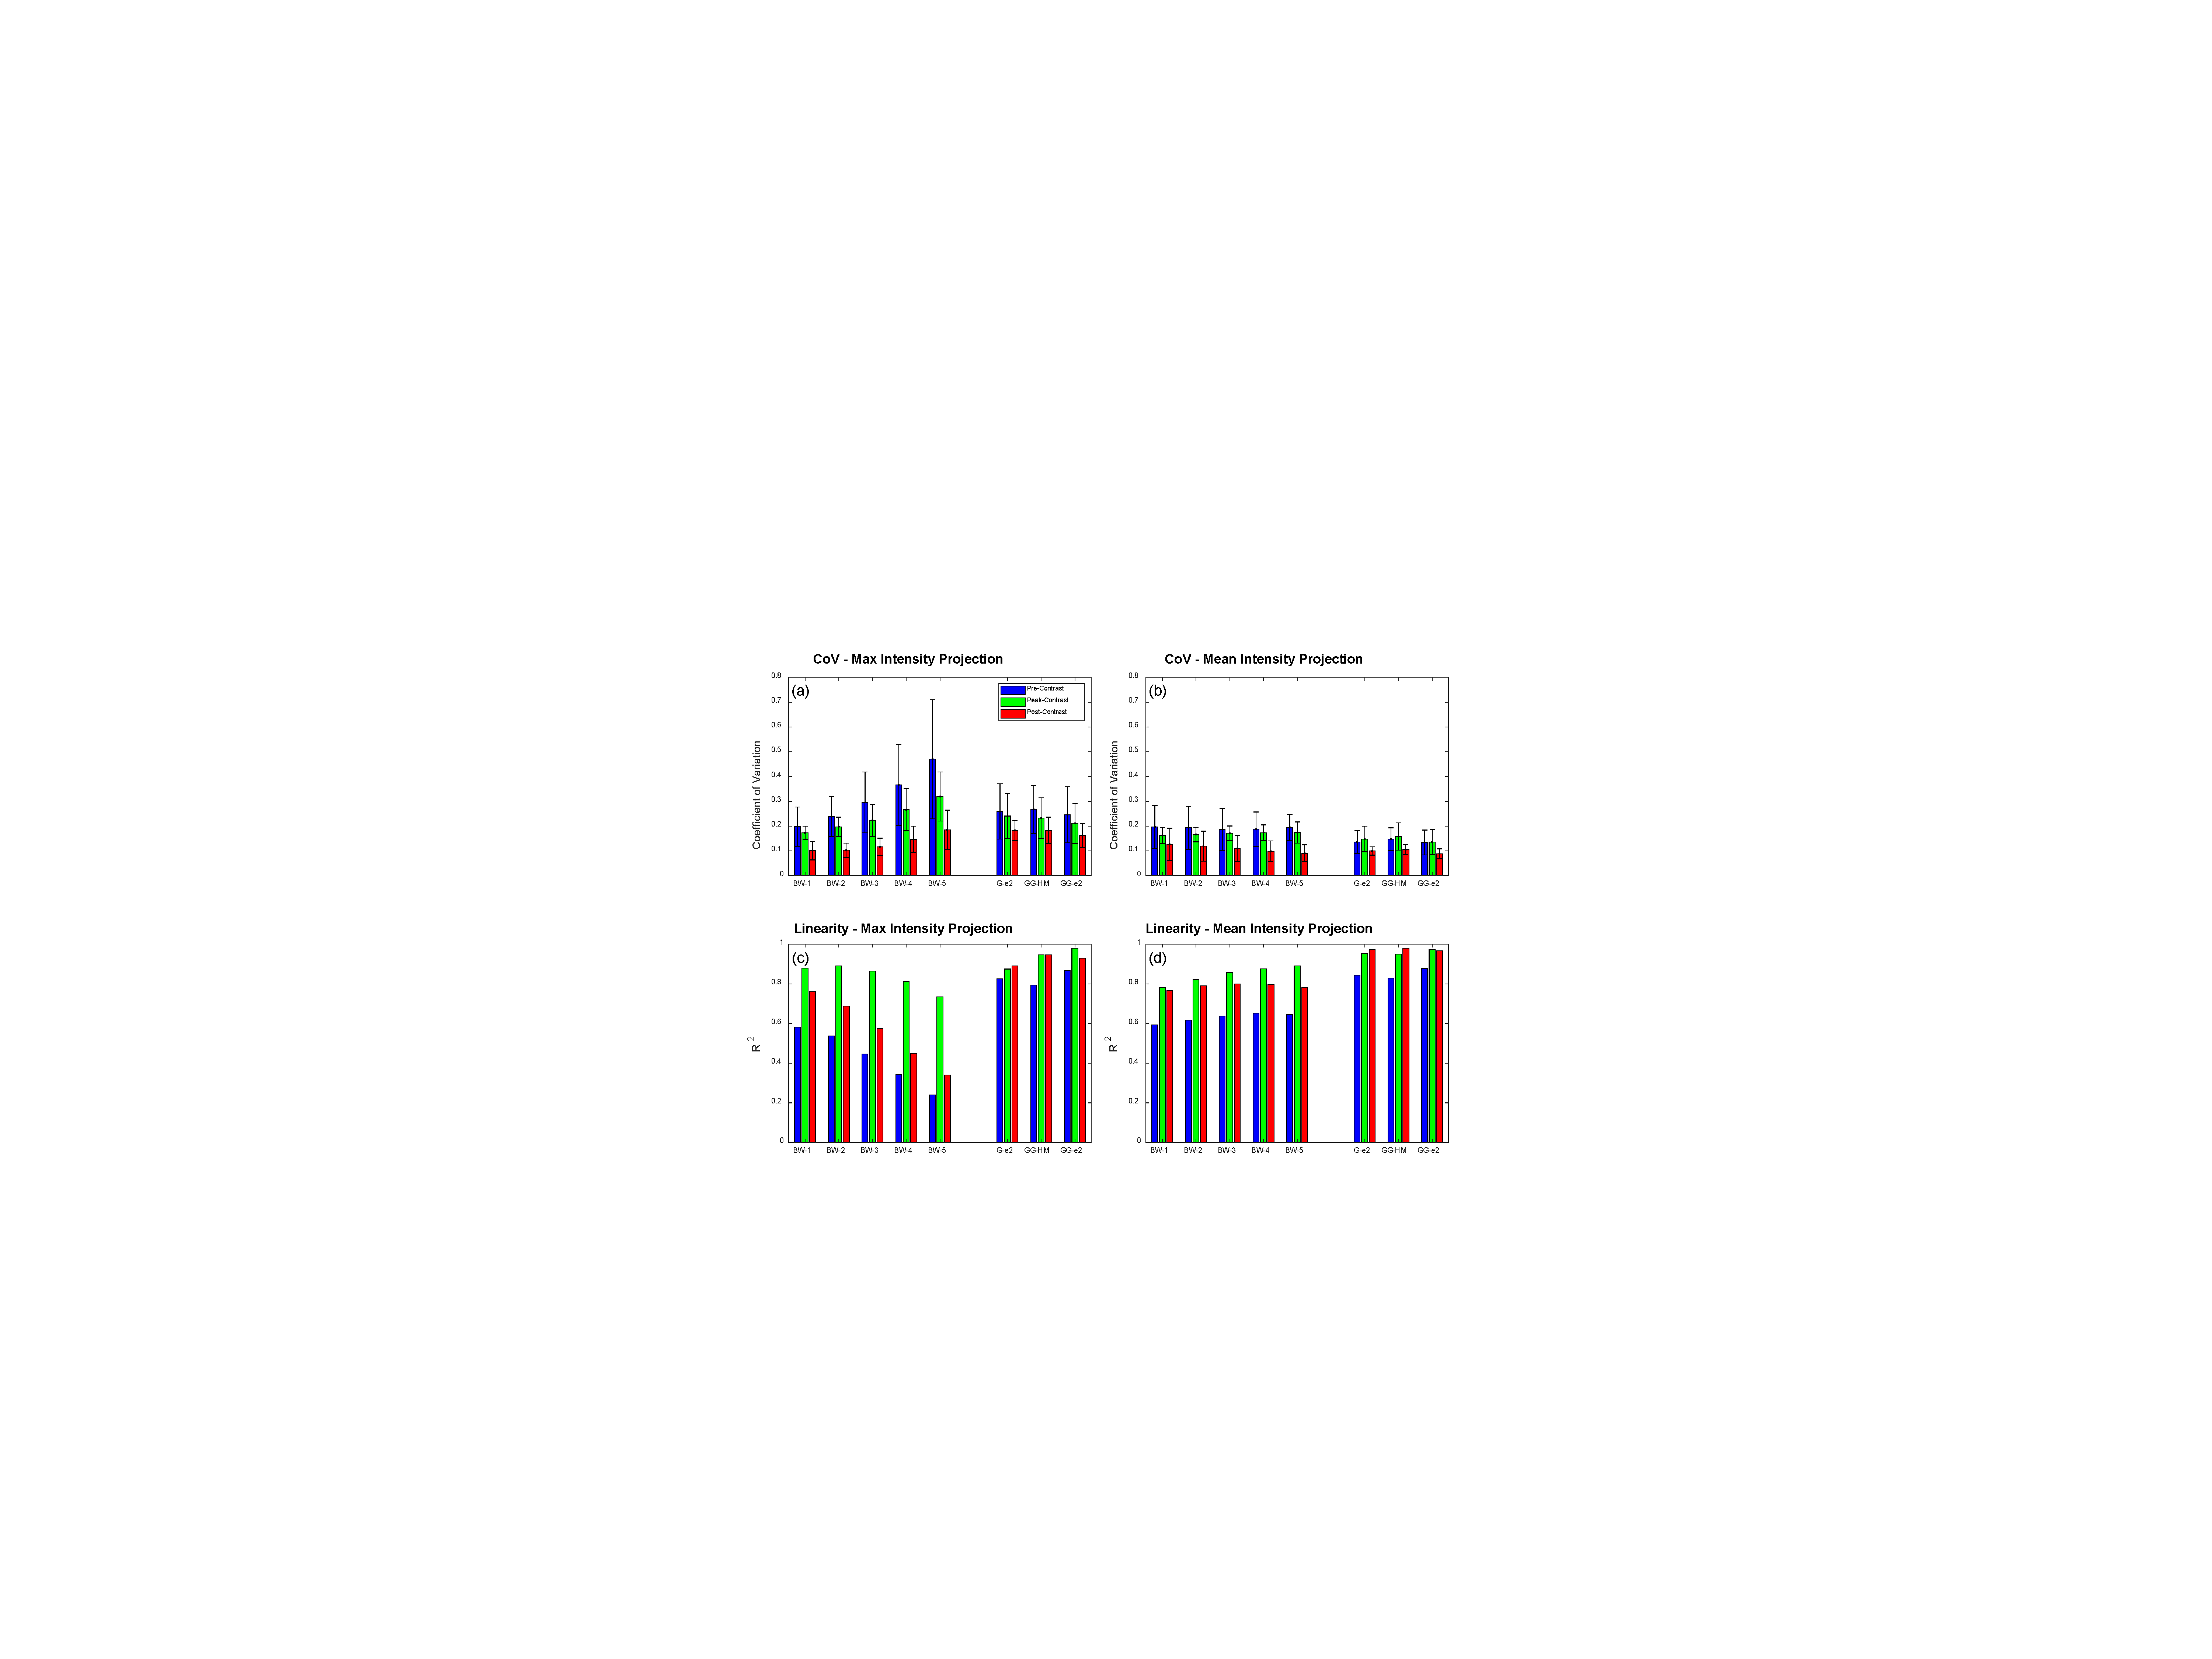
\includegraphics[width=\linewidth,height=\dimexpr\textheight-\pagetotal-10\baselineskip\relax,keepaspectratio]{figures/Figure_7.pdf}
\caption{Summary of repeatability and linearity across all diameter measurement methods. (a,b) Coefficient of variation (CoV) for MIP and MeIP, respectively. (c,d) Coefficient of determination ($R^2$) for MIP and MeIP, respectively. Bars are grouped by method (BW-1 through BW-5, G-$e^2$, GG-HM, GG-$e^2$) and colour-coded by contrast condition: pre-contrast (blue), peak-contrast (green), and post-contrast (red). Model based methods consistently show lower CoV and higher $R^2$ than binarisation based methods.}
\label{fig:cov_r2}
\end{figure}

\subsection{Functional flicker stimulation}
\label{subsec:flicker}
To investigate whether the choice of diameter measurement method affects the detection of physiological vascular responses, functional flicker stimulation was performed in a C57BL/6 mouse and vessel diameter was measured before and after photoreceptor stimulation using each of the three approaches (Fig.~\ref{fig:flicker}).

The Gaussian and GG model-based time series (Figs.~\ref{fig:flicker}a,b) showed visible diameter increases following stimulation onset for most of the five vessels examined, consistent with the expected neurovascular coupling-driven vasodilation. The binarised angiogram time series (Fig.~\ref{fig:flicker}c), however, showed the opposite trend: a paradoxical decrease in measured diameter following stimulation. Bar charts summarising the mean pre- and post-stimulation diameters per vessel (Figs.~\ref{fig:flicker}d--f) confirmed this pattern. For the Gaussian model, four of five vessels showed significant diameter increases ($p < 0.01$), with percentage changes of $+9.2\%$, $+9.6\%$, $+28.5\%$, and $+4.9\%$ for vessels 1, 2, 4, and 5, respectively (Fig.~\ref{fig:table}). The GG model similarly detected significant increases in three of five vessels ($+9.9\%$, $+28.4\%$, and $+3.1\%$ for vessels 2, 4, and 5). In marked contrast, the binarised method detected significant diameter \emph{decreases} in four of five vessels ($-12.5\%$, $-10.2\%$, $-4.2\%$, and $-9.3\%$ for vessels 1, 2, 3, and 5).

\begin{figure}[H]
\centering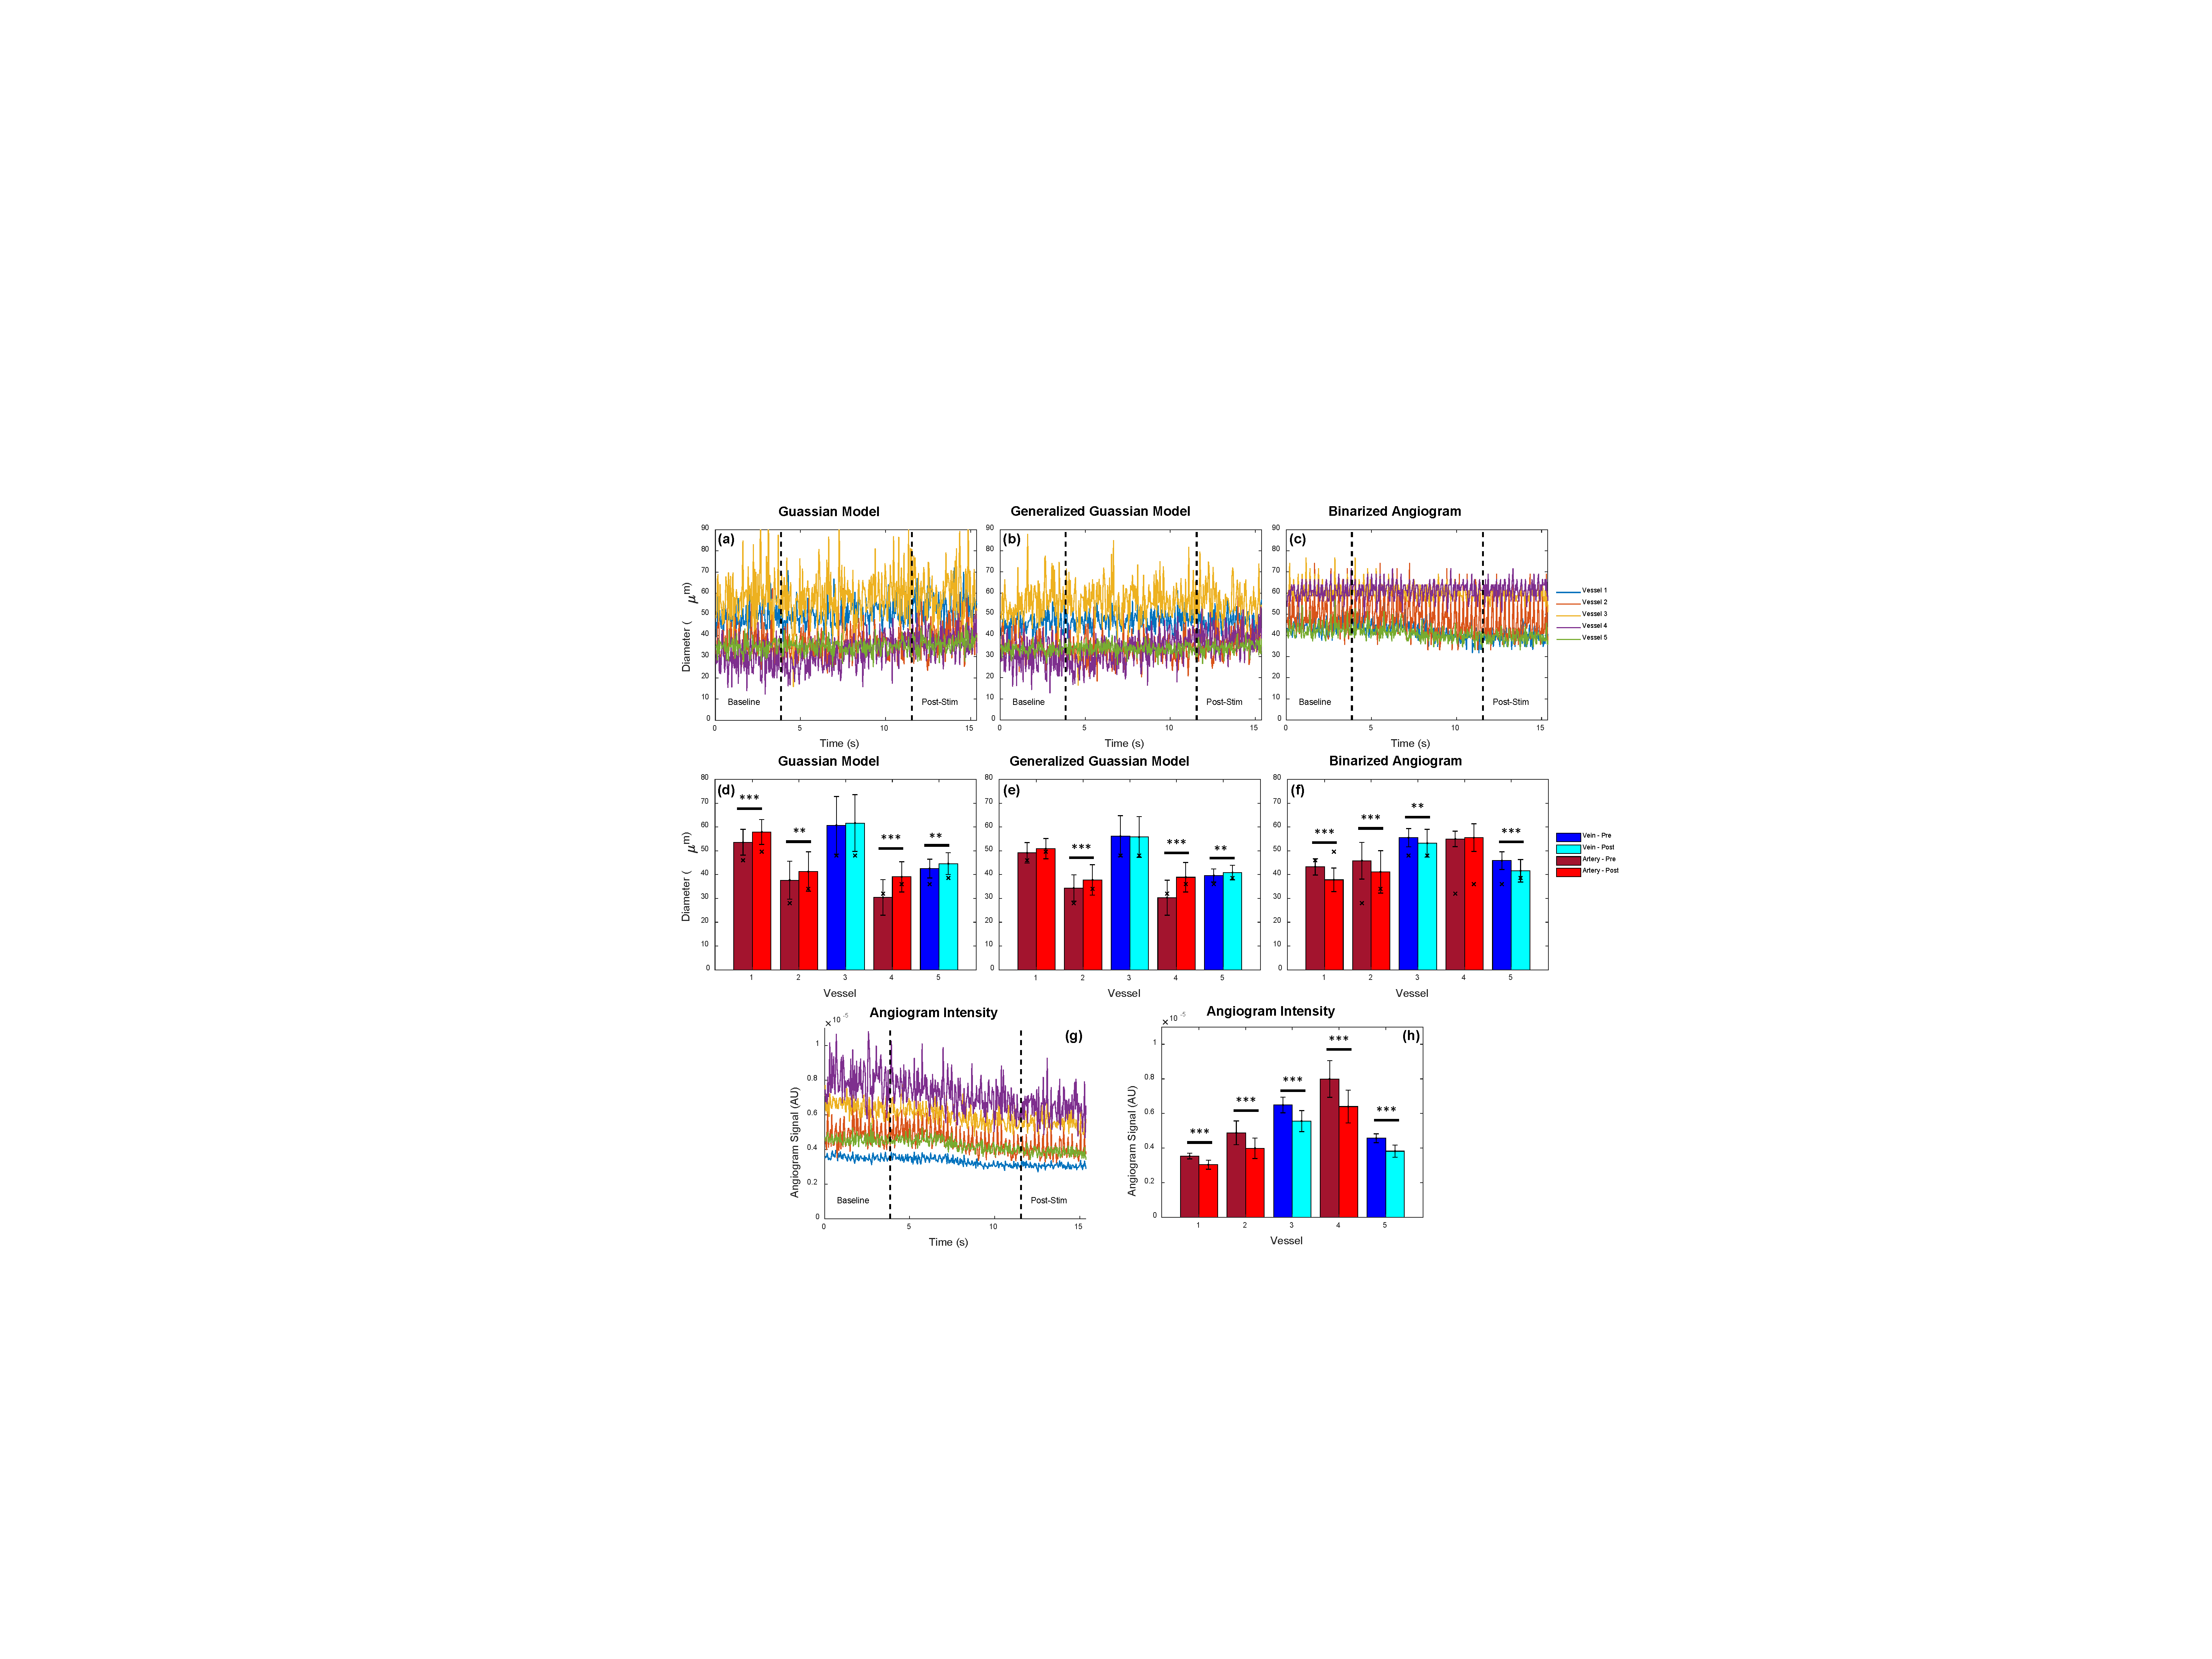
\includegraphics[width=\linewidth,height=\dimexpr\textheight-\pagetotal-14\baselineskip\relax,keepaspectratio]{figures/Figure_8.pdf}
\caption{Functional flicker stimulation results. (a--c) Time series of vessel diameter during baseline and post-stimulation periods for (a) Gaussian model, (b) generalised Gaussian model, and (c) binarised angiogram, across five vessels. Dashed lines indicate stimulation onset and offset. (d--f) Mean diameter per vessel before (dark bars) and after (light bars) stimulation for each method; veins are shown in blue/cyan and arteries in dark/light red. Significance levels: $^{**}p < 0.01$, $^{***}p < 0.001$. (g) Angiogram signal intensity time series and (h) mean intensity per vessel before and after stimulation. Model-based methods detect the expected vasodilation, whereas the binarised method paradoxically reports vasoconstriction.}
\label{fig:flicker}
\end{figure}

The explanation for this paradoxical binarisation result lies in the concomitant change in angiogram signal intensity. Following stimulation, the angiogram intensity decreased significantly for all five vessels ($p < 0.0005$), with reductions ranging from $-14.1\%$ to $-19.9\%$ (Figs.~\ref{fig:flicker}g,h; Fig.~\ref{fig:table}). Because the binarised diameter is derived from the number of pixels exceeding a fixed threshold, a reduction in signal intensity directly translates to fewer above-threshold pixels and hence a smaller apparent diameter, even if the true vessel diameter has increased.

To quantify this confounding, the correlation between diameter change and angiogram intensity change was computed for each method (Table~\ref{fig:table}). For the binarised method, the per-vessel correlations were uniformly positive and strong ($\rho = 0.59$, $0.80$, $0.27$, $0.46$, $0.52$ for vessels 1--5), yielding an overall correlation of $\rho = 0.523$ ($p < 0.0005$). This indicates that the binarised diameter measurement is substantially confounded by the angiogram signal intensity. In contrast, the Gaussian model yielded an overall correlation of $\rho = -0.101$ and the GG model yielded $\rho = -0.098$, confirming that the model-based diameter measurements are effectively independent of angiogram signal intensity fluctuations. These results demonstrate that model-based fitting not only provides more accurate and repeatable diameter measurements, but also recovers physiologically meaningful vascular responses that binarisation-based methods can misrepresent.

\begin{table}[htbp]
\caption{Summary of flicker stimulation results. Top: percentage diameter change per vessel for each method together with corresponding $p$-values. Bottom: Pearson correlation ($\rho$) between measured diameter and angiogram signal intensity for each method and vessel. Overall correlations: Gaussian $= -0.101$, GG $= -0.098$, BW $= 0.523$.}
\label{fig:table}
\centering
\resizebox{\textwidth}{!}{%
\begin{tabular}{l c c c c c c c c c c}
\hline
\textbf{Change in Diameter} & \multicolumn{2}{c}{\textbf{Vessel 1}} & \multicolumn{2}{c}{\textbf{Vessel 2}} & \multicolumn{2}{c}{\textbf{Vessel 3}} & \multicolumn{2}{c}{\textbf{Vessel 4}} & \multicolumn{2}{c}{\textbf{Vessel 5}} \\
\hline
Gaussian (\% Change) & \textbf{9.2} & $p < 0.0005$ & \textbf{9.6} & $p = 0.0019$ & 1.5 & $p = 0.59$ & \textbf{28.5} & $p < 0.0005$ & \textbf{4.9} & $p = 0.0008$ \\
Gen.\ Gaussian (\% Change) & 1.5 & $p = 0.28$ & \textbf{9.9} & $p < 0.0005$ & $-0.6$ & $p = 0.79$ & \textbf{28.4} & $p < 0.0005$ & \textbf{3.1} & $p = 0.0034$ \\
Binarised (\% Change) & $\mathbf{-12.5}$ & $p < 0.0005$ & $\mathbf{-10.2}$ & $p < 0.0005$ & $\mathbf{-4.2}$ & $p = 0.0011$ & 1.0 & $p = 0.404$ & $\mathbf{-9.3}$ & $p < 0.0005$ \\
Angiogram Intensity (\% Change) & $\mathbf{-14.1}$ & $p < 0.0005$ & $\mathbf{-18.2}$ & $p < 0.0005$ & $\mathbf{-14.3}$ & $p < 0.0005$ & $\mathbf{-19.9}$ & $p < 0.0005$ & $\mathbf{-16.3}$ & $p < 0.0005$ \\
\hline
\\[-0.5em]
\hline
\textbf{Correlation to Intensity} & \multicolumn{2}{c}{\textbf{Vessel 1}} & \multicolumn{2}{c}{\textbf{Vessel 2}} & \multicolumn{2}{c}{\textbf{Vessel 3}} & \multicolumn{2}{c}{\textbf{Vessel 4}} & \multicolumn{2}{c}{\textbf{Vessel 5}} \\
\hline
Gaussian Diameter Corr.\ & $-0.07$ & $p = 0.48$ & \textbf{0.23} & $p = 0.019$ & $\mathbf{-0.28}$ & $p = 0.0044$ & $-0.15$ & $p = 0.14$ & $\mathbf{-0.24}$ & $p = 0.018$ \\
Gen.\ Gaussian Diameter Corr.\ & 0.03 & $p = 0.79$ & 0.07 & $p = 0.47$ & $\mathbf{-0.28}$ & $p = 0.0056$ & $-0.14$ & $p = 0.16$ & $-0.18$ & $p = 0.081$ \\
Binarised Diameter Corr.\ & \textbf{0.59} & $p < 0.0005$ & \textbf{0.80} & $p < 0.0005$ & \textbf{0.27} & $p = 0.0077$ & \textbf{0.46} & $p < 0.0005$ & \textbf{0.52} & $p < 0.0005$ \\
\hline
\end{tabular}%
}
\end{table}
% ~\FloatBarrier~%print all pending figures/tables right here, don’t let them move past this point.